\documentclass[10pt,twocolumn]{article}
% Shared two-column preamble for the three research papers.
% Use with: \documentclass[10pt,twocolumn]{article}
% Then in main.tex: % Shared two-column preamble for the three research papers.
% Use with: \documentclass[10pt,twocolumn]{article}
% Then in main.tex: % Shared two-column preamble for the three research papers.
% Use with: \documentclass[10pt,twocolumn]{article}
% Then in main.tex: \input{../../shared/latex/twocolumn_preamble.tex}

\usepackage[margin=0.75in]{geometry}
\usepackage[utf8]{inputenc}
\usepackage[T1]{fontenc}
\usepackage{lmodern}
\usepackage{microtype}
\usepackage{amsmath,amssymb,amsthm}
\usepackage{graphicx}
\usepackage{booktabs}
\usepackage{caption}
\usepackage{subcaption}
\usepackage{hyperref}
\usepackage{url}
\usepackage{xcolor}
\usepackage{algorithm}
\usepackage{algorithmic}
\usepackage{multirow}
\usepackage{titlesec}
\usepackage{authblk}

\hypersetup{colorlinks=true,linkcolor=blue!50!black,citecolor=blue!50!black,urlcolor=blue!50!black}

\titleformat{\section}{\normalfont\large\bfseries}{\thesection}{0.6em}{}
\titleformat{\subsection}{\normalfont\bfseries}{\thesubsection}{0.5em}{}

\captionsetup{font=small,labelfont=bf,skip=4pt}
\setlength{\columnsep}{0.25in}
\setlength{\parskip}{2pt}

\newtheorem{theorem}{Theorem}
\newtheorem{proposition}[theorem]{Proposition}
\newtheorem{definition}[theorem]{Definition}


\usepackage[margin=0.75in]{geometry}
\usepackage[utf8]{inputenc}
\usepackage[T1]{fontenc}
\usepackage{lmodern}
\usepackage{microtype}
\usepackage{amsmath,amssymb,amsthm}
\usepackage{graphicx}
\usepackage{booktabs}
\usepackage{caption}
\usepackage{subcaption}
\usepackage{hyperref}
\usepackage{url}
\usepackage{xcolor}
\usepackage{algorithm}
\usepackage{algorithmic}
\usepackage{multirow}
\usepackage{titlesec}
\usepackage{authblk}

\hypersetup{colorlinks=true,linkcolor=blue!50!black,citecolor=blue!50!black,urlcolor=blue!50!black}

\titleformat{\section}{\normalfont\large\bfseries}{\thesection}{0.6em}{}
\titleformat{\subsection}{\normalfont\bfseries}{\thesubsection}{0.5em}{}

\captionsetup{font=small,labelfont=bf,skip=4pt}
\setlength{\columnsep}{0.25in}
\setlength{\parskip}{2pt}

\newtheorem{theorem}{Theorem}
\newtheorem{proposition}[theorem]{Proposition}
\newtheorem{definition}[theorem]{Definition}


\usepackage[margin=0.75in]{geometry}
\usepackage[utf8]{inputenc}
\usepackage[T1]{fontenc}
\usepackage{lmodern}
\usepackage{microtype}
\usepackage{amsmath,amssymb,amsthm}
\usepackage{graphicx}
\usepackage{booktabs}
\usepackage{caption}
\usepackage{subcaption}
\usepackage{hyperref}
\usepackage{url}
\usepackage{xcolor}
\usepackage{algorithm}
\usepackage{algorithmic}
\usepackage{multirow}
\usepackage{titlesec}
\usepackage{authblk}

\hypersetup{colorlinks=true,linkcolor=blue!50!black,citecolor=blue!50!black,urlcolor=blue!50!black}

\titleformat{\section}{\normalfont\large\bfseries}{\thesection}{0.6em}{}
\titleformat{\subsection}{\normalfont\bfseries}{\thesubsection}{0.5em}{}

\captionsetup{font=small,labelfont=bf,skip=4pt}
\setlength{\columnsep}{0.25in}
\setlength{\parskip}{2pt}

\newtheorem{theorem}{Theorem}
\newtheorem{proposition}[theorem]{Proposition}
\newtheorem{definition}[theorem]{Definition}

\newcommand{\SceneBlades}{200}
\newcommand{\SceneTris}{800}
\newcommand{\BigBlades}{1{,}600}
\newcommand{\BigTris}{6{,}400}
\newcommand{\BruteTestsBig}{31{,}987{,}980}
\newcommand{\BvhTestsBig}{237{,}949}
\newcommand{\AccelSpeedup}{134}
\newcommand{\AccelSpeedupInst}{149}
\newcommand{\MemRatio}{3}
\newcommand{\BvhSpeedupRender}{41}
\newcommand{\InstSpeedupRender}{47}
\newcommand{\McSlope}{-0.43}
\newcommand{\RefSpp}{24}
\newcommand{\SsimOneSpp}{0.708}
\newcommand{\SsimOneSppDn}{0.747}
\newcommand{\DenoiseGainOne}{3.9}
\newcommand{\LodSimpFloor}{0.973}
\newcommand{\LodBillFloor}{0.949}
\newcommand{\LodCostFloor}{80}
\newcommand{\StackSsim}{0.908}
\newcommand{\StackSpeedup}{277}
\newcommand{\BvhRelCostPct}{2.4}


\title{Ray Tracing on a Budget: Measuring the Cost of Zelda's Grass Trick
and Three Other Ways to Trace Fewer Rays}
\author[1]{Luis Benvenuto}
\affil[1]{Independent Research}
\date{\today}

\begin{document}
\twocolumn[
\maketitle
\begin{@twocolumnfalse}
\begin{abstract}
\noindent Ray tracing is expensive because every ray is tested, independently,
against the scene's geometry --- which is why photoreal rendering wants very
capable GPUs. Games do not pay that bill in full: \emph{The Legend of Zelda:
Breath of the Wild} did not treat every blade of grass as unique geometry, it
replicated one blade and instanced it, and faded distant detail to a cheaper
form. We build a from-scratch path tracer whose cost is measured in
machine-independent ray/primitive tests, and use it to quantify four ways to
trace fewer rays against an exact high-sample reference. Two are lossless: a
bounding-volume hierarchy (BVH) and geometry instancing (the grass trick) cut
intersection tests by \AccelSpeedup$\times$ and \AccelSpeedupInst$\times$ on our
largest scene while producing a \emph{bit-identical} image. Two are lossy: level
of detail and a Monte-Carlo sample budget rescued by a normal/depth-guided
denoiser, each buying further speedups at a quality price we read off directly
(Monte-Carlo error falls with the theoretical $N^{-1/2}$ slope,
$\McSlope$ measured). Placing every method on a single cost--quality plane, the
lossless methods move the frontier for free and the lossy methods trade a
measurable amount of structural similarity for another order of magnitude of
cost: the full stack reaches SSIM $\StackSsim$ at \StackSpeedup$\times$ less cost
than brute force. The grass trick is not an approximation --- it is free, and the
right question is what to spend the savings on.
\end{abstract}
\vspace{1em}
\end{@twocolumnfalse}
]

\section{Introduction}
\label{sec:intro}

Ray tracing produces images by simulating light transport: for each pixel a ray
is cast into the scene and tested against geometry, and the rays that matter ---
shadows, reflections, indirect bounces --- spawn more rays
\cite{whitted1980improved, kajiya1986rendering}. The method is physically
principled and embarrassingly parallel, but it is also expensive in a very
literal sense: cost scales with the number of ray/primitive intersection tests,
and a naive renderer tests every ray against every primitive. A field of grass,
where each blade is a handful of triangles and there are tens of thousands of
blades, is exactly the kind of scene that makes this bill explode, which is why
real-time ray tracing waits on ever more capable GPUs.

Games do not pay the bill in full. \emph{The Legend of Zelda: Breath of the
Wild} is famous for its rolling grass, and it did not achieve that by treating
every blade as unique, independently simulated geometry. It stored essentially
one blade and \emph{replicated} it thousands of times as cheap transformed
copies, and it faded distant grass to simpler stand-ins. These are two of the
oldest ideas in rendering --- instancing and level of detail --- and they are the
starting point for this paper: \emph{how much does each trick actually save, and
what, if anything, does it cost in image quality?}

We answer this with a deliberately self-contained tool: a from-scratch path
tracer, a few hundred lines of numpy, whose cost we measure not only in
wall-clock time but in \emph{ray/primitive intersection tests} --- a
machine-independent currency that is reproducible on any computer. On one
canonical scene (a procedural grass field with a few spheres under a sun) we
study four ways to trace fewer rays:

\begin{enumerate}
\item \textbf{Bounding-volume hierarchy (BVH).} A spatial tree so a ray tests
  only nearby primitives. Lossless: the image is unchanged.
\item \textbf{Instancing} --- the grass trick. One canonical blade, many affine
  transforms, a two-level hierarchy. Lossless: the image is unchanged, but the
  geometry is stored once.
\item \textbf{Level of detail (LOD).} Distant blades collapse to a single
  triangle or a flat billboard. Lossy: the image changes, measurably.
\item \textbf{Sample budget and denoising.} Fewer Monte-Carlo samples per pixel
  (cheaper, noisier), rescued by a normal/depth-guided denoiser. Lossy.
\end{enumerate}

Our contribution is measurement rather than a new algorithm. We (i) confirm the
two lossless methods are lossless --- bit-identical images --- and quantify their
savings and how they scale with scene size; (ii) chart the quality price of the
two lossy methods against an exact reference using PSNR and SSIM
\cite{wang2004image}; and (iii) place all of them on a single cost--quality
Pareto frontier, so the ``opportunity cost'' of each shortcut, and the way they
compose, can be read off one plot. The headline is simple: the grass trick is
not an approximation, it is free; the interesting decisions begin only after you
have spent the free savings.

\section{Related work}
\label{sec:related}

\paragraph{Ray tracing and path tracing.} Whitted's recursive ray tracing
\cite{whitted1980improved} introduced shadows, reflection, and refraction by
spawning secondary rays; Kajiya's rendering equation \cite{kajiya1986rendering}
cast image synthesis as an integral over all light paths, solved by Monte-Carlo
path tracing. Our tracer is a minimal path tracer (direct sun plus one diffuse
bounce), enough to exhibit both the geometric cost that acceleration structures
attack and the stochastic noise that sample budgets and denoisers attack. The
ray/triangle test is Möller--Trumbore \cite{moller1997fast}; the standard
reference for the whole pipeline is \emph{Physically Based Rendering}
\cite{pharr2016physically}.

\paragraph{Acceleration structures.} The idea that a ray should not be tested
against every primitive dates to the earliest complex-scene renderers
\cite{rubin1980representation}. Bounding-volume hierarchies are now the dominant
structure, including for dynamic scenes \cite{wald2007ray} and in hardware
ray-tracing cores. We use a textbook median-split BVH; our interest is not in a
better build but in \emph{measuring} what it buys.

\paragraph{Instancing.} Storing one mesh and referencing it through many
transforms --- a two-level hierarchy with a bottom-level structure (BLAS) per
mesh and a top-level structure (TLAS) over instances --- is standard in production
and is the mechanism behind dense vegetation such as the grass of \emph{Breath of
the Wild}. It is lossless by construction; we verify this and quantify its cost
and memory savings.

\paragraph{Level of detail.} Replacing distant geometry with cheaper
approximations is a classic real-time technique \cite{luebke2003level}; billboard
impostors are its aggressive limit. Unlike the lossless methods, LOD changes the
image, and the quality/cost trade is exactly what we measure.

\paragraph{Sampling and denoising.} Monte-Carlo estimators converge as
$N^{-1/2}$ in the number of samples, so halving noise costs four times the rays.
Learned and hand-built denoisers \cite{chaitanya2017interactive} make low-sample
renders usable and underpin production systems (e.g.\ NVIDIA OptiX, DLSS). Our
denoiser is a cross-bilateral filter \cite{tomasi1998bilateral} guided by
G-buffer normals and depth --- the minimal version of that idea, chosen so its
behaviour is transparent rather than opaque.

\section{Method}
\label{sec:method}

\subsection{Scene and renderer}
The canonical scene is a procedural grass field: a jittered grid of blades on a
ground plane, with a few coloured spheres, lit by a single directional sun over
a gradient sky. Each blade is a canonical shape in local space (four triangles
at full detail) placed by an affine transform $x \mapsto Ax + b$ encoding
position, yaw, tilt, and height. Everything is deterministic given a seed. Our
rendered scene uses \SceneBlades\ blades (\SceneTris\ triangles) at
$64\times48$; the accompanying \texttt{gpu\_full} config scales this up without
code changes.

The renderer is a Monte-Carlo path tracer: a primary ray per pixel (jittered for
anti-aliasing), a shadow ray to the sun, and one cosine-weighted diffuse bounce
whose contribution is estimated from direct light at the second hit or the sky.
Averaging $N$ samples per pixel (spp) reduces variance. A deterministic centre
ray also records a G-buffer (albedo, normal, depth) used by the denoiser.

\subsection{Cost as a currency}
We report cost as the count of \emph{ray/primitive intersection tests}
(triangle, sphere, plane, and bounding-box tests), incremented by every routine
that performs one. Unlike wall-clock time, this is exact and machine
independent. For the acceleration study we count the tests to cast one primary
plus one shadow ray per pixel; for the Pareto study we use
\begin{equation}
\text{cost}(\text{method}, N) \;=\; \text{tests}_{\text{1 pass}} \times N,
\end{equation}
a single currency that combines geometric cost (the intersection structure) with
sampling cost (spp), normalised so brute force at the reference sample count is
$1$.

\subsection{The four techniques}
\paragraph{Brute force (baseline).} Every ray is tested against every triangle:
$O(\text{rays}\times\text{triangles})$.

\paragraph{BVH.} A median-split bounding-volume hierarchy over triangle
centroids. A ray descends the tree, testing a box before its subtree and only
reaching the few triangles in leaves it cannot rule out. The image is identical
to brute force; only the test count changes.

\paragraph{Instancing.} A two-level BVH: the canonical blade is stored once as a
BLAS, and each blade is an instance in a TLAS. A ray is transformed into an
instance's local frame ($A^{-1}(o-b)$, $A^{-1}d$, without renormalising $d$ so
the hit distance $t$ is preserved) and tested against the shared blade. Geometry
is stored once rather than duplicated $K$ times; the image is bit-identical.

\paragraph{Level of detail.} Beyond a distance threshold, a blade is baked with a
cheaper shape --- a single triangle (\emph{simplified}) or a flat two-triangle
card (\emph{billboard}). The threshold in $[0,1]$ is the fraction of the
camera-distance range kept at full detail; lower means cheaper and more
approximate.

\paragraph{Sample budget and denoising.} We sweep spp and, at each, apply a
cross-bilateral denoiser whose weights combine spatial distance, colour
similarity, and geometric similarity (normal agreement to the eighth power and a
depth term), so it smooths noise within a surface without blurring across
silhouettes.

\subsection{Metrics}
Quality is measured against a high-sample reference (\RefSpp\ spp) with PSNR and
windowed SSIM \cite{wang2004image}, both implemented in numpy. Lossless methods
attain SSIM $=1$ by construction (verified to floating-point in the tests);
lossy methods produce a curve.

\section{Lossless acceleration}
\label{sec:accel}

\begin{figure*}[t]
\centering
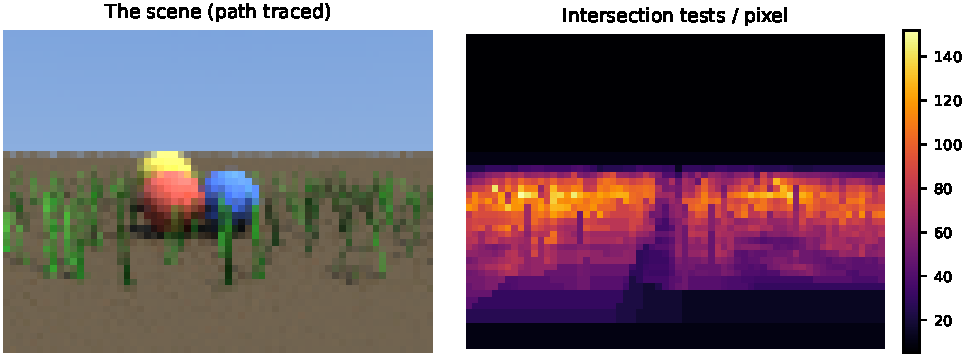
\includegraphics[width=\textwidth]{figures/scene_cost.pdf}
\caption{Left: the canonical scene, path traced. Right: intersection tests per
pixel for a primary-plus-shadow ray. The grass dominates the cost budget ---
exactly the geometry the lossless tricks target.}
\label{fig:scene}
\end{figure*}

\begin{figure*}[t]
\centering
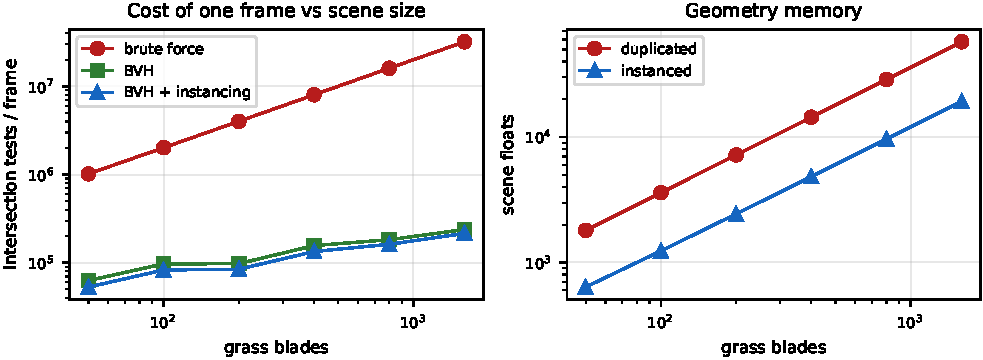
\includegraphics[width=\textwidth]{figures/accel_scaling.pdf}
\caption{Left: intersection tests to render one frame as the grass field grows.
Brute force is linear in triangle count; the BVH and instancing are far flatter.
Right: geometry memory --- instancing stores one blade plus per-instance
transforms instead of duplicated triangles.}
\label{fig:accel}
\end{figure*}

Figure~\ref{fig:scene} shows where a frame's cost goes: the per-pixel test count
is concentrated on the grass, which is why accelerating grass is the whole game.
Both lossless methods produce an image \emph{identical} to brute force --- we
verify bit-for-bit equality in the unit tests (BVH versus brute; instancing
versus duplicated geometry) --- so their only effect is on the test count.

\paragraph{BVH.} Brute force tests every ray against every triangle, and
Figure~\ref{fig:accel} (left) shows the resulting linear growth: on our largest
field (\BigBlades\ blades, \BigTris\ triangles) a primary-plus-shadow pass costs
\BruteTestsBig\ tests. The BVH cuts this to \BvhTestsBig, a
\AccelSpeedup$\times$ reduction, and the gap widens with scene size because the
BVH cost grows roughly logarithmically in the number of primitives. On the
smaller rendered scene the lossless BVH speedup is \BvhSpeedupRender$\times$; the
factor is not a constant but a function of how much geometry the structure lets
each ray skip.

\paragraph{Instancing.} Instancing adds a second win. In test count it edges out
the flat BVH (\AccelSpeedupInst$\times$ versus \AccelSpeedup$\times$ on the large
scene) because the shared blade BVH is tiny and cache-friendly to traverse. Its
real advantage, though, is memory: Figure~\ref{fig:accel} (right) contrasts
storing $K$ duplicated blades against one blade plus $K$ cheap transforms. With
our deliberately tiny four-triangle blade the memory ratio is only
\MemRatio$\times$, because a $3\times3$-plus-translation transform ($12$ floats)
is not much smaller than four triangles ($36$ floats); the ratio grows towards
the blade's triangle count for realistic vegetation with hundreds of triangles
per blade. This is the honest shape of the grass trick: for the geometry Nintendo
was drawing, instancing turns a prohibitive memory footprint into a trivial one,
and it does so for free in image quality.

The lesson of this section is that a large part of ray tracing's cost is simply
\emph{waste} --- testing rays against geometry they could never hit --- and that
removing it changes nothing about the picture. Only after this free lunch do real
trade-offs begin.

\section{Lossy shortcuts and their price}
\label{sec:lossy}

\begin{figure*}[t]
\centering
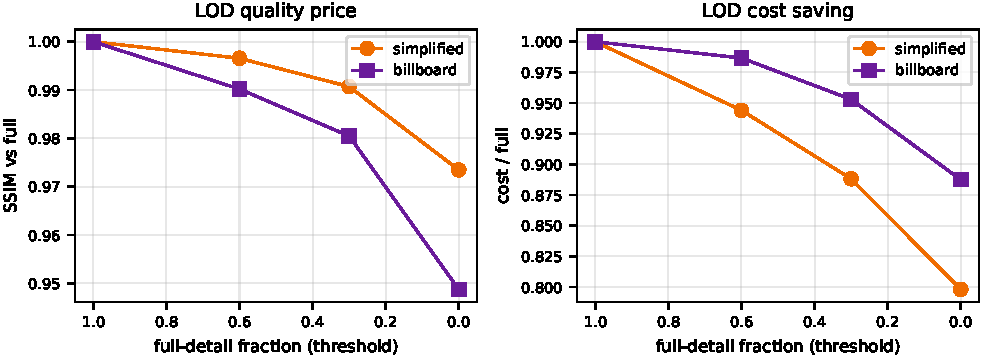
\includegraphics[width=\textwidth]{figures/lod_curve.pdf}
\caption{Level of detail. Left: SSIM against the full-detail image as more of
the field is simplified (threshold decreasing to the right). Right: the matching
cost fraction. Billboards are cheaper but degrade quality faster than the
single-triangle simplification.}
\label{fig:lod}
\end{figure*}

\begin{figure*}[t]
\centering
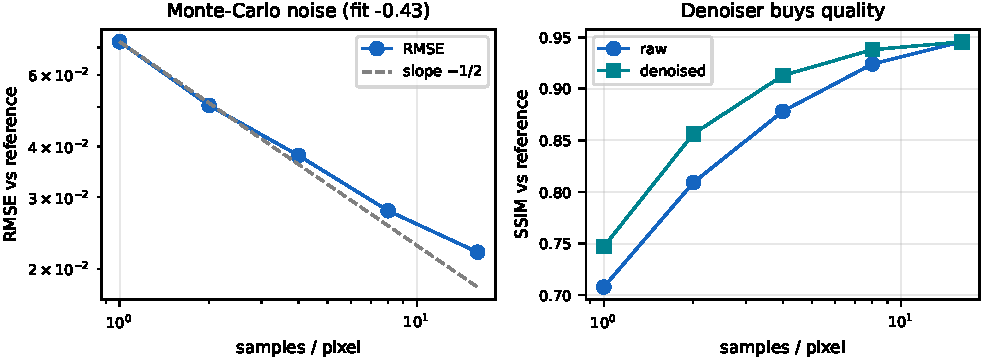
\includegraphics[width=\textwidth]{figures/sampling.pdf}
\caption{Sample budget. Left: RMSE against the reference versus samples per
pixel, tracking the theoretical $N^{-1/2}$ slope (fit \McSlope). Right: SSIM
with and without the guided denoiser --- the denoiser helps most where noise is
worst, at low sample counts.}
\label{fig:sampling}
\end{figure*}

Unlike Section~\ref{sec:accel}, the next two techniques change the image, so the
question becomes how much quality each unit of saved cost costs.

\paragraph{Level of detail.} Figure~\ref{fig:lod} sweeps the distance threshold
from all-full to all-simplified. Collapsing every far blade to a single triangle
holds SSIM at \LodSimpFloor\ --- a barely perceptible change --- while the flat
billboard, cheaper still, falls to \LodBillFloor. The striking part is the cost
axis: the saving is modest (down to \LodCostFloor\% of full-detail cost), far
smaller than the geometry reduction. The reason is precisely the previous
section: once a BVH is in place, halving the triangle count barely moves
traversal cost, because most of that cost is boxes, not triangles. LOD's classic
payoff --- fewer triangles to store, transform, and rasterise --- is a memory and
front-end win; inside a ray tracer with a good BVH, it is a weak lever on
intersection cost. That is a result worth stating plainly, and it reframes when
LOD is and is not the right tool.

\paragraph{Sample budget and denoising.} The stochastic side behaves as theory
predicts: Figure~\ref{fig:sampling} (left) shows RMSE falling with the
$N^{-1/2}$ Monte-Carlo slope (measured \McSlope), so quality here is bought by
brute-force sampling at a punishing exchange rate. The denoiser changes the
rate. At one sample per pixel it lifts SSIM from \SsimOneSpp\ to \SsimOneSppDn\
(a \DenoiseGainOne-point gain) by exploiting the noise-free G-buffer to smooth
within surfaces without crossing edges; the benefit shrinks as samples rise and
the image is already clean, exactly as it should. A cheap spatial filter guided
by geometry is worth several times its cost in samples in the noisy regime ---
the principle, in miniature, behind production denoisers.

\section{The cost--quality frontier}
\label{sec:results}

\begin{figure}[t]
\centering
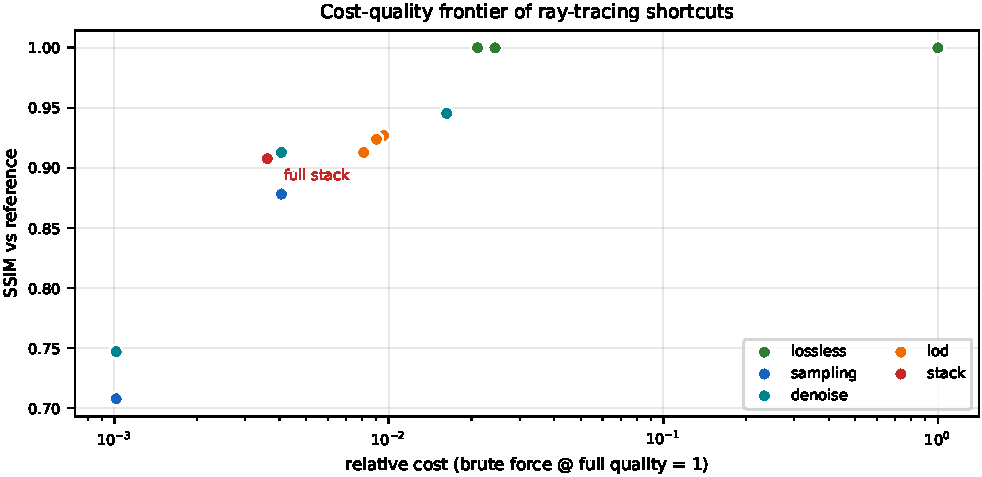
\includegraphics[width=\columnwidth]{figures/pareto.pdf}
\caption{Every technique on one plane: relative cost (log scale, brute force at
full quality $=1$) versus SSIM against the reference. Lossless methods sit at
SSIM $1$ and move left for free; lossy methods trade quality for another order
of magnitude of cost. The full stack combines instancing, LOD, few samples, and
denoising.}
\label{fig:pareto}
\end{figure}

Figure~\ref{fig:pareto} collects the whole study on a single cost--quality
plane. Three things stand out.

First, the two lossless methods are a vertical wall at SSIM $=1$: they buy
\BvhSpeedupRender--\InstSpeedupRender$\times$ (rising with scene size) at zero
quality loss. Any renderer should take this before considering anything else; a
BVH takes brute force from relative cost $1$ to \BvhRelCostPct\% of it with an
identical picture.

Second, the lossy methods extend the frontier by another order of magnitude but
now bend downward in quality. The sample-budget points trace the Monte-Carlo
curve; the denoised points sit above them at equal cost, pushing the frontier up
and to the left. LOD points, by contrast, sit in an awkward region: on this scene,
with a BVH already in place, they save little cost for their quality cost, so
they are Pareto-dominated by simply rendering fewer samples and denoising. This
is scene- and renderer-specific --- LOD earns its keep when geometry, not
sampling, is the bottleneck --- but it is a concrete reminder that a technique's
value depends on what else is already switched on.

Third, the methods compose. The full stack --- instancing for memory, LOD
geometry, four samples per pixel, and the guided denoiser --- reaches SSIM
\StackSsim\ at \StackSpeedup$\times$ less cost than the brute-force reference.
Most of that factor comes from the free, lossless layers; the lossy layers
contribute the last stretch at a quality cost one can see on the plot and decide
whether to pay.

The practical reading is a priority order. Structure first (BVH, instancing):
free, always worth it, and the larger the scene the larger the win. Then spend
the sampling budget where it matters and lean on a geometry-guided denoiser to
stretch it. Reach for LOD when the geometry --- not the noise --- is what is
actually costing you. The ``opportunity cost'' the introduction asked about is,
in the end, legible: it is the vertical drop on Figure~\ref{fig:pareto} you
accept in exchange for each horizontal step left.

\section{Limitations and conclusion}
\label{sec:conclusion}

\paragraph{Limitations.} This is a measurement study on a toy, not a renderer to
ship. The tracer is pure numpy on a CPU, so absolute times are irrelevant --- we
deliberately report machine-independent intersection tests instead, but that
currency ignores memory bandwidth, cache behaviour, SIMD/GPU divergence, and the
hardware BVH traversal that dominates real systems. The scene is a single grass
field with one bounce of diffuse global illumination; reflection, refraction,
and deep light paths --- where ray tracing's cost and its advantage over
rasterisation truly live --- are absent. The BVH is a plain median split, not the
surface-area-heuristic builds used in practice, and the denoiser is a single
bilateral pass rather than a temporal or learned reconstructor. Finally, the LOD
result (that it saves little intersection cost once a BVH exists) is specific to
a geometry-light, sampling-heavy regime; a scene with far more geometry per pixel
would shift that balance. Every one of these is a knob in the \texttt{gpu\_full}
config or a natural extension, not a rewrite.

\paragraph{Conclusion.} We measured, against an exact reference, four standard
ways to trace fewer rays. The two lossless ones --- a BVH and the instancing
trick behind \emph{Breath of the Wild}'s grass --- cut intersection tests by one
to two orders of magnitude while leaving the image bit-identical, and their
advantage grows with scene size. The two lossy ones --- level of detail and a
denoised sample budget --- extend the frontier further at a quality price we
quantified with SSIM and PSNR, and we showed they compose into a stack that is
\StackSpeedup$\times$ cheaper than brute force at SSIM \StackSsim. The most
useful output is not any single number but the ordering it implies: take the free
lossless savings first, spend samples and denoise second, and reach for
approximation last and deliberately, knowing exactly what each shortcut costs.
Ray tracing is expensive, but a large part of that expense is avoidable without
compromise --- and the rest is a trade you can price.


\bibliographystyle{plain}
\bibliography{references}

\end{document}
